% ========== Appendix B

\chapter{Treatment Specifications for the Drink Area}
\label{chap:appendix_drinkTreatments}
%\begin{figure}[ht!]
%\centering
%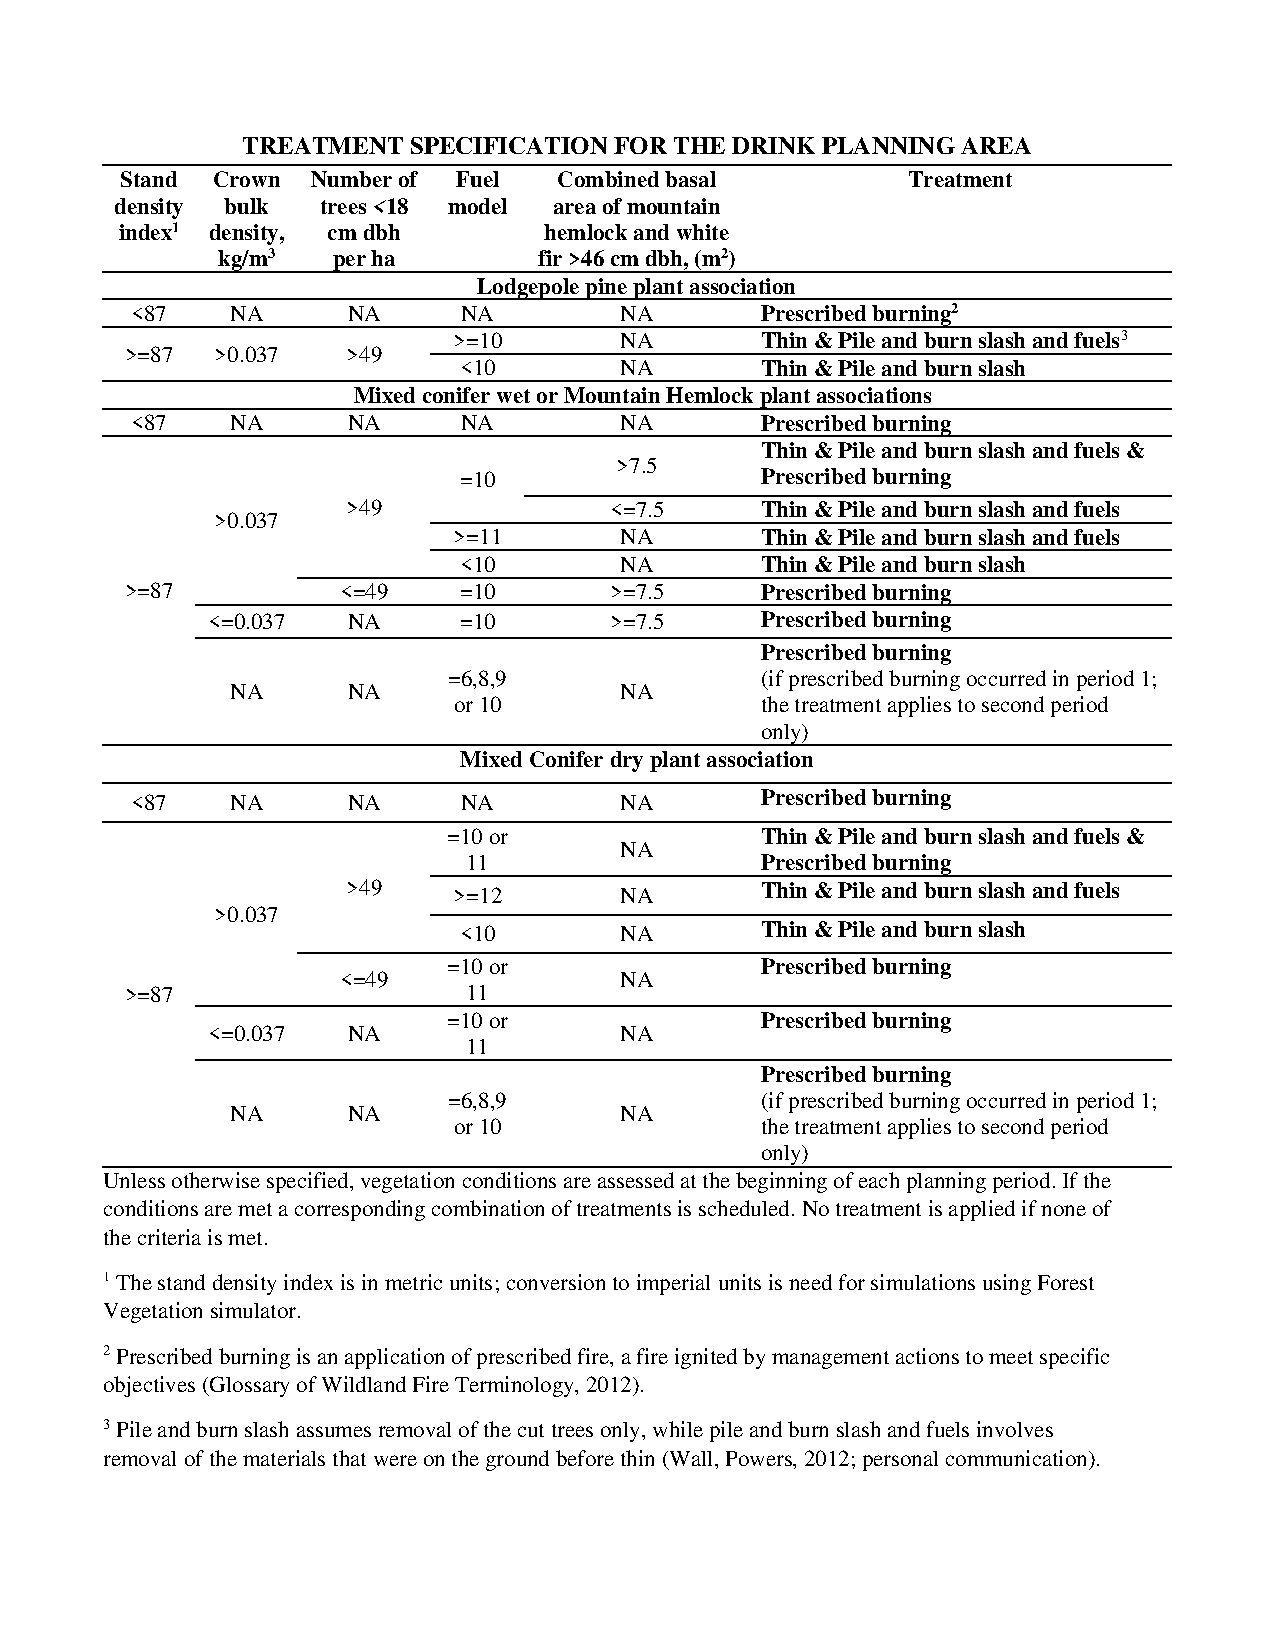
\includegraphics[width=\textwidth]{./appB/TreatmentSpecsForDrink.pdf}
%\end{figure}
%=-,scale=0.5,pagecommand=\subsection{blub}]{./appB/TreatmentSpecsForDrink.pdf}

Table \ref{tab:drinkTreatmentRules} provides a mapping from a treatment unit's vegetation conditions to the type of fuels removal to apply to the treatment unit. If a treatment unit's conditions do not correspond to any row in the table, then no action is taken. The table was adapted from Schroder \cite{schroder2016multi}. The plant association groups in the Drink area are shown in Figure \ref{fig:drinkPAGs}.

\begin{longtable}{p{.1\linewidth}p{.1\linewidth}p{.15\linewidth}p{.15\linewidth}p{.2\linewidth}p{.25\linewidth}}
\caption[Rules governing treatment assignments in the Drink.]{Rules governing treatment assignments.} \\
\label{tab:drinkTreatmentRules}\\
\hline
\textbf{SDI}\footnote{Stand Density Index, calculated in metric units (trees per ha).}    & \textbf{CBD}\footnote{Crown bulk density ($kg/m^3$)}   & \textbf{$\text{TPH}_{<18}$}\footnote{Number of trees per hectare whose diameter at breast height (DBH) is less than 18 cm}       & \textbf{Fuel model}\footnote{According to the Anderson rating system\cite{anderson1982aids}}  & $\text{\textbf{BA}}_{\text{MHD+WF,}>46}$\footnote{Basal area in $m^2$ of all mountain hemlock (MHD) and white fir (WF) trees with DBH $> 46 cm$.} & \textbf{Treatment}                                                                \\ \hline
\multicolumn{6}{c}{\textbf{Lodgepole pine (LPD) plant association}}                                                                                                                                                                                                                                                                                                   \\ \hline
$<87$                      & N/A                                                    & N/A                                                 & N/A                  & N/A                                                                                                     & \textbf{Prescribed burn}                                                        \\ \hline
\multirow{2}{*}{$\ge 87$}  & \multirow{2}{*}{$>0.037$}                     & \multirow{2}{*}{$> 49$}                    & $ \ge 10$       & N/A                                                                                                     & \textbf{Thin, pileburn slash and fuels}\footnote{Pileburning slash involves removal of thinned trees only, while pileburning slash and fuels also involves removal of materials that were on the ground before thinning (Wall, Powers, 2012; personal communication)}                                         \\ \cline{4-6} 
                                  &                                                        &                                                     &$< 10$         & N/A                                                                                                     & \textbf{Thin, pileburn slash}                                                     \\ \hline
\multicolumn{6}{c}{\textbf{Mixed conifer wet (MCW) or mountain hemlock (MHD) plant associations}}                                                                                                                                                                                                                                                                     \\ \hline
$<87$                       & N/A                                                    & N/A                                                 & N/A                  & N/A                                                                                                     & \textbf{Prescribed burn}                                                          \\ \hline
\multirow{7}{*}{$\ge 87$}  & \multirow{5}{*}{$>0.037$}                     & \multirow{4}{*}{$>49$}                     & \multirow{2}{*}{$=10$} & $>7.5$                                                                                         & \textbf{Thin, pileburn slash and fuels, prescribed burn}                          \\ \cline{5-6} 
                                  &                                                        &                                                     &                      & $ \le 7.5$                                                                                          & \textbf{Thin, pileburn slash and fuels}                                           \\ \cline{4-6} 
                                  &                                                        &                                                     & $>10$       & N/A                                                                                                     & \textbf{Thin, pileburn slash and fuels}                                           \\ \cline{4-6} 
                                  &                                                        &                                                     & $< 10$         & N/A                                                                                                     & \textbf{Thin, pileburn slash}                                                     \\ \cline{3-6} 
                                  &                                                        & $ \le 49$                                       & $=10$                  & $ \ge 7.5$                                                                                       & \textbf{Prescribed burn}                                                          \\ \cline{2-6} 
                                  & $ \le 0.037$                                        & N/A                                                 & $=10$                  & $\ge 7.5$                                                                                        & \textbf{Prescribed burn}                                                          \\ \cline{2-6} 
                                  & N/A                                                    & N/A                                                 & $\in \{6,8,9,10\}$            & N/A                                                                                                     & \textbf{Prescribed burn}\footnote{\label{footnote:p2TrtNote}Only if prescribed burn was assigned in period 1 (applies to period 2 treatment assignments only)} \\ \hline
\multicolumn{6}{c}{\textbf{Mixed conifer dry (MCD) plant association}}                                                                                                                                                                                                                                                                                                \\ \hline
$<87$                       & N/A                                                    & N/A                                                 & N/A                  & N/A                                                                                                     & \textbf{Prescribed burn}                                                          \\ \hline
\multirow{6}{*}{$ \ge 87$} & \multicolumn{1}{c}{\multirow{4}{*}{$ > 0.037$}} & \multicolumn{1}{c}{\multirow{3}{*}{$ >49$}} & $\in \{10,11\}$               & N/A                                                                                                     & \textbf{Thin, pileburn slash and fuels, prescribed burn}                          \\ \cline{4-6} 
                                  & \multicolumn{1}{c}{}                                   & \multicolumn{1}{c}{}                                & $\ge 12$      & N/A                                                                                                     & \textbf{Thin, pileburn slash and fuels}                                           \\ \cline{4-6} 
                                  & \multicolumn{1}{c}{}                                   & \multicolumn{1}{c}{}                                & $ < 10$          & N/A                                                                                                     & \textbf{Thin, pileburn slash}                                                     \\ \cline{3-6} 
                                  & \multicolumn{1}{c}{}                                   & $ \le 49$                                        & $\in \{10,11\}$               & N/A                                                                                                     & \textbf{Prescribed burn}                                                          \\ \cline{2-6} 
                                  & $\le 0.037$                                        & N/A                                                 & $\in \{10,11\}$               & N/A                                                                                                     & \textbf{Prescribed burn}                                                          \\ \cline{2-6} 
                                  & N/A                                                    & N/A                                                 & $\in \{6,8,9,10\}$            & N/A                                                                                                     & \textbf{Prescribed burn}\footnotemark[\ref{footnote:p2TrtNote}] \\
%\end{tabular}
\end{longtable}
%\end{table}

\begin{figure}
\centering
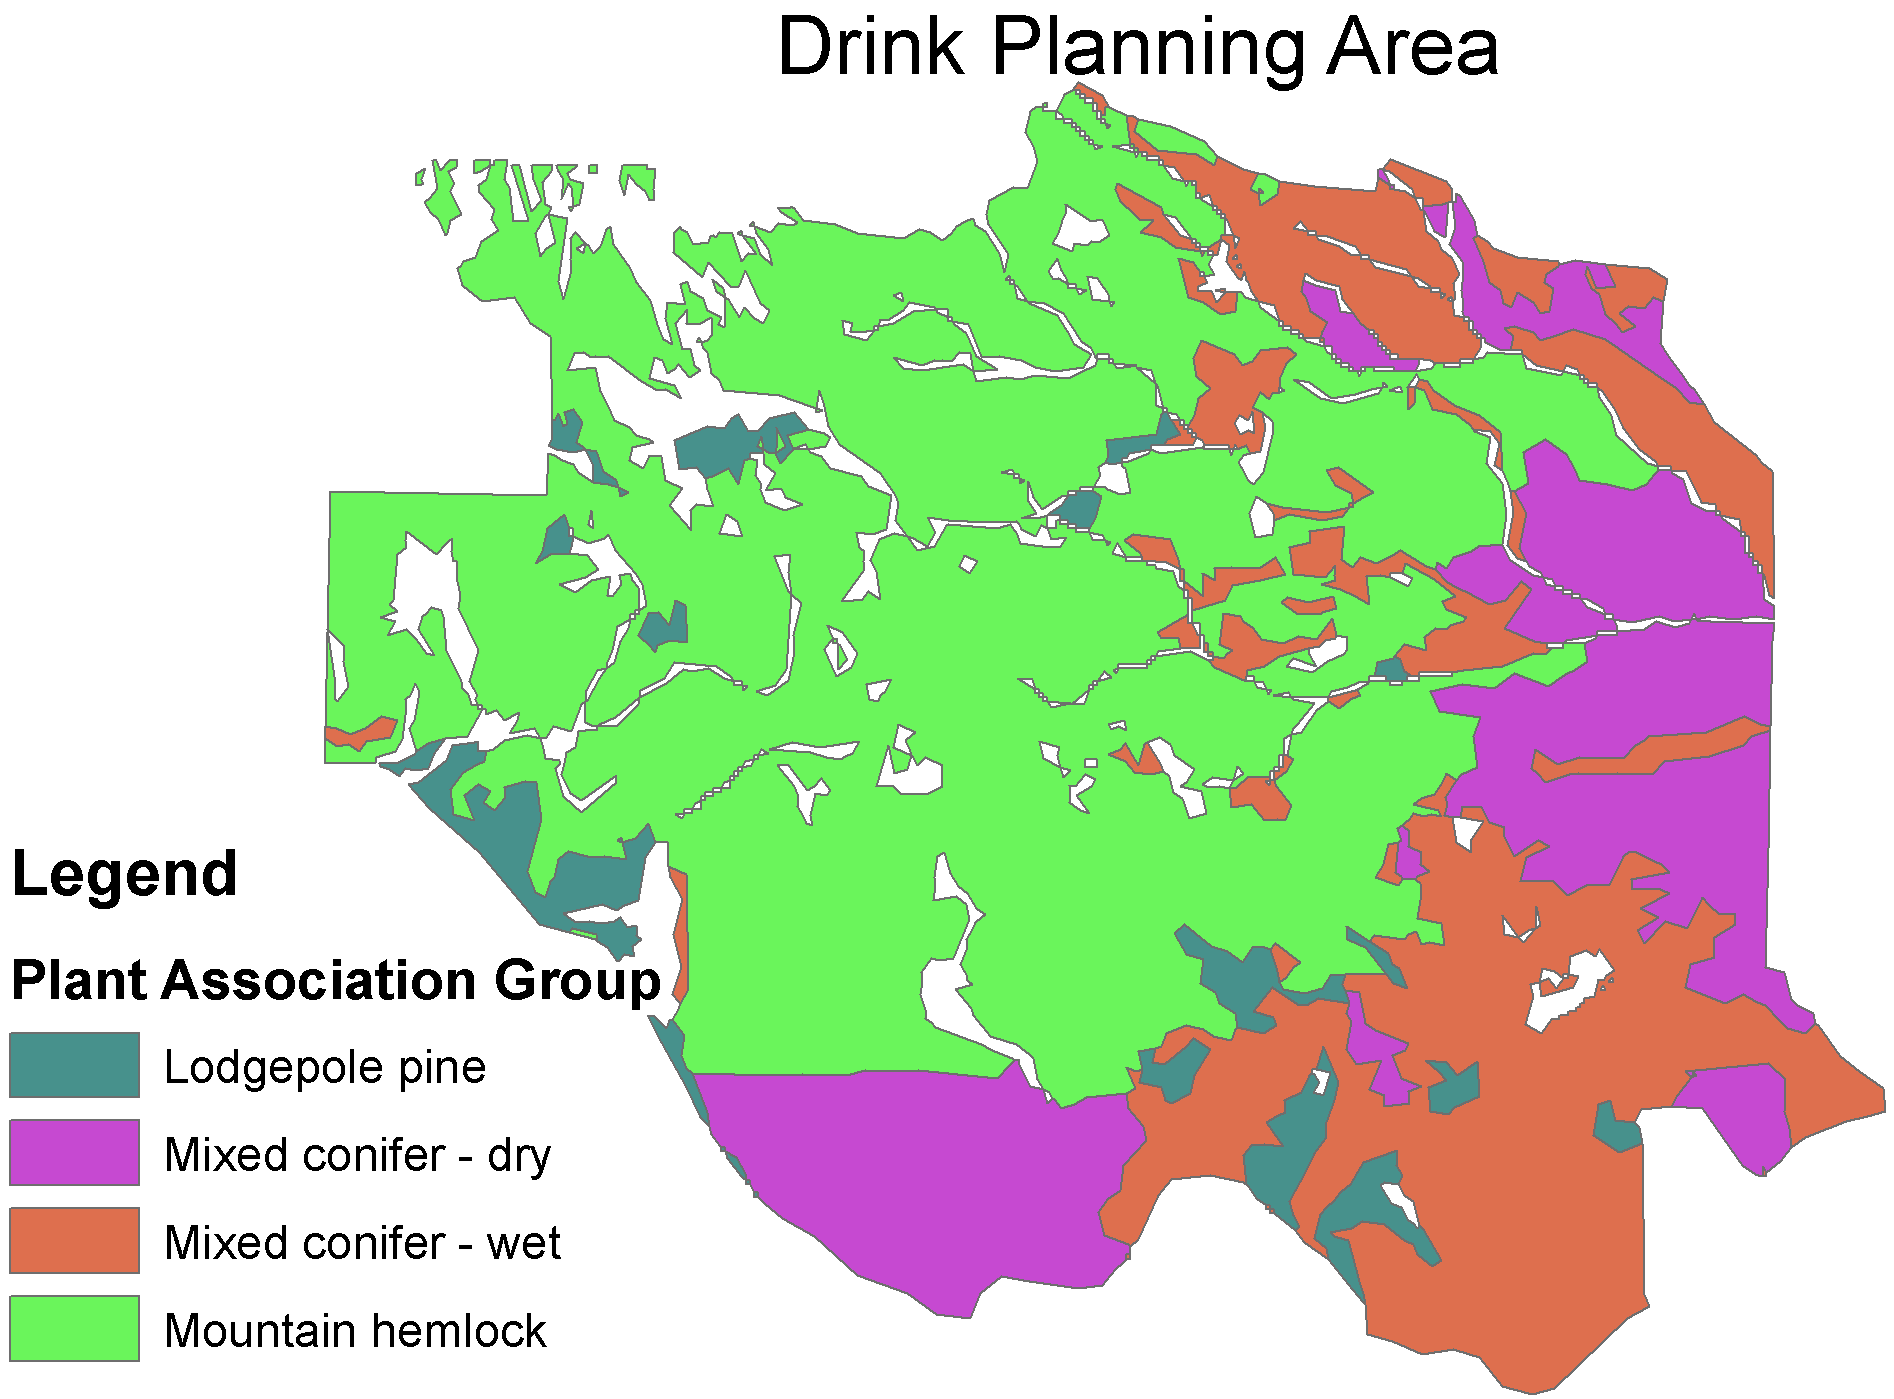
\includegraphics[width=.5\textwidth]{../images/DrinkMap_PAGs}
\caption[Plant association groups in the Drink Planning Area]{Plant association groups in the Drink Area that are considered for treatments.}
\label{fig:drinkPAGs}
\end{figure}